\chapter{Market Risk}
\label{chap:MarketRisk}

\section{Market Risk}



\section{Market Risk Metrics}

\section{The Computational Burden of Market Risk Computations}

\section{Market Risk as a Supervised Machine Learning Problem}

\section{Model Scores for Market Risk}

\section{Unsupervised Machine Learning Alternatives}
\subsection{Deep Learning}
\subsection{Differential Deep Learning}
\subsection{Other}

\newpage

\section{A Base Case Example}

As a base case example we will use an option for which a closed form solution exists. This will allow us compare the results obtained by a supervised machine learning algorithm to those obtained by the closed form formula.

In order to add both non linear features and the possibility of increasing the dimension of the problem, we will use a call option on the geometric mean of a basket.

\begin{equation}\label{eq:geom_digital}
\begin{aligned}
&V_{T}=\max\left(G_T-k,0\right) \\
&G_{T}=\left(\prod_{j=1}^{m} \frac{S_{T}^{j}}{S_{0}^{j}}\right)^{1 / m} \\
\end{aligned}
\end{equation}

Where $S_t^1,\ldots,S_t^m$ represent the prices of the underlying assets as of time t and $G_T$ represents the geometric mean of one plus the return of the different assets from time $0$ to time $T$. $T$ represents the option's payoff date.

We will assume geometric Brownian motion dynamics for the different underlying assets under the risk neutral measure:

\begin{equation}\label{eq:geom_brownianmotion}
\frac{S_{T}^{j}}{S_{t}^{j}}=\exp\left(\left(r-q_{j}-\frac{\sigma_{j}^{2}}{2}\right) \left( T - t\right)+\sigma_{j} \left(W_{T}^{j}-W_{t}^{j}\right)\right)
\end{equation}

Where $r$ represents the risk free rate, $q_j$ the continuous dividend yield , $\sigma_j$ the volatility and $W_T^j$ the change experienced form $0$ to $T$ of a Brownian motion. The $j$ index help us distinguish the parameters of the different underlying assets.

Taking into account \ref{eq:geom_brownianmotion}

\begin{equation}\label{eq:geom_digital_distrib}
\left(\prod_{j=1}^m\frac{S_{T}^{j}}{S_{0}^{j}}\right)^{\frac{1}{m}} &=\left(\prod_{j=1}^m\frac{S_{t}^{j}}{S_{0}^{j}}\right)^{\frac{1}{m}}\exp\left(\frac{1}{m} \sum_{j=1}^{m}\left(r-q_{j}-\frac{\sigma_{j}^{2}}{2}\right) \left(T-t\right)+\frac{1}{m} \sum_{j=1}^{m} \sigma_{j} \left(W_{T}^{j}-W_{t}^{j}\right)\right) 
\end{equation}

Notice that $G_T$, conditional on $S_t^1,\cdots,S_t^m$ is log-normally distributed with parameters:



\begin{equation} 
\label{eq:geom_digital_distrib_params1}
\begin{aligned} 
& G_T|\mathcal{F}_t \eqdistr A \exp\left(\mu+\Sigma\phi\right)\\
& A = \left(\prod_{j=1}^m\frac{S_{t}^{j}}{S_{0}^{j}}\right)^{\frac{1}{m}} \\
&\mu = \frac{1}{m}\sum_{j=1}^{m}\left(r-q_{j}-\frac{\sigma_{j}^{2}}{2}\right)T \\   
& \Sigma=\frac{1}{m}\sqrt{\sigma^{\top} C_{w} \sigma}
\end{aligned}
\end{equation}

Where $\eqdistr$ represents equal in distribution, $\mathcal{F}_t$ the market filtration as of time $t$,$\sigma$ is a column vector containing the volatilities of the different underlying assets, $C_W$ the covariance matrix of $W_T^1,\cdots,W_T^m$ and $\phi$ is a standard normal distributed random variable.

\begin{equation} \label{eq:geom_digital_distrib_params2}
\begin{aligned}
&\sigma=\left[\begin{array}{c}
\sigma_{1} \\
\vdots \\
\sigma_{m}
\end{array}\right] \\
&C_{w}=\left[\begin{array}{cccc}
\left(T-t\right) & \rho_{12} \left(T-t\right) & \cdots & \rho_{1 m} \left(T-t\right) \\
\vdots & \vdots & & \vdots \\
\rho_{m 1} \left(T-t\right) & \rho_{m 2} \left(T-t\right) & \cdots &  \left(T-t\right)
\end{array}\right]
\end{aligned}
\end{equation} 

$\rho_{ij}$ represents the correlation of $W_t^i$ and $W_t^j$.

Given the distribution of $G_T$, the pricing formula as of time $t<T$ will be given by:

$$
\begin{array}{lll}
V_{t}&=&\exp (-r(T-t)) E_{\mathbb{Q}}\left[1_{\{G_{T}>K\}} | \mathcal{F}_t\right] \\
&& \\
&=&\left(A\exp\left(\mu+\frac{\Sigma^2}{2}\right)N\left(d_1\right)-k\left(d_2\right)\right)\exp\left(-r(T-t)\right)
\end{array}
$$

$$
\begin{aligned}
d_1 = \frac{\log\frac{A\exp\left(\mu+\frac{\Sigma^2}{2}\right)}{K}+\frac{\Sigma^2}{2}}{\Sigma} \\
d_2 = \frac{\log\frac{A\exp\left(\mu+\frac{\Sigma^2}{2}\right)}{K}-\frac{\Sigma^2}{2}}{\Sigma} \\
\end{aligned}
$$


% $$
% & E_{\mathbb{Q}}\left[1_{\{G_{T}>K\}} | \mathcal{F}_t\right]=P\left[Ae^{\mu+\sum \phi}>k\right] \\
% & =P\left[\phi<\frac{\log \frac{A}{K}+\mu}{\Sigma}\right]=N\left(\frac{\log \frac{A}{K}+\mu}{\Sigma}\right)
% \end{aligned}
% $$

Where $\phi$ represents a standard normal random variable and $N$ its cumulative distribution function. $\mathbb{Q}$ represents the risk neutral measure.


\subsection{Unhedged Portfolio}
 In this section we will explore how the usage of machine learning techniques perform while trying to represent the payoff function in isolation. Nevertheless, we should keep in mind that it is common to perform market risk calculations for trading portfolios where exotics payoffs as the one introduced in the last section are hedged with vanilla instruments. This is the reason why in the next section we will tackle the hedged portfolio case. 
 
 As payoff function we will use call option on the geometric mean of a basket with two underlying assets $\{A,B\}$. We will use the following product characteristics:
 
\begin{center}
\begin{tabular}{||c | c||} 
 \hline
 Time to maturity $(T-t)$ & 3 years \\
 \hline
 $S_0^A$ & $1.0$ \\
 \hline
 $S_0^B$ & $1.0$ \\
 \hline
 $K$ & $1.0$ \\
 \hline
 \end{tabular}
\end{center}

And these are the values for market variables (model parameters):

\begin{center}
\begin{tabular}{||c | c||} 
 \hline
 $S_t^A$ & 1.0 \\
 \hline
 $S_t^B$ & 1.0 \\
 \hline
 $\sigma_t^A$ & $0.2$ \\
 \hline
 $\sigma_t^B$ & $0.3$ \\
 \hline
 $r$ & $0.01$ \\
 \hline
 $q_A$ & $0.0$ \\
 \hline
 $q_B$ & $0.0$ \\
 \hline
 $rho$ & $0.8$ \\
 \hline
\end{tabular}
\end{center}

We will apply market risk scenarios to $S_t^A,\ S_t^B,\ \sigma_t^A,\ \sigma_t^B$.
In order to apply market risk scenarios we make use of historical data for both the spot prices and the $1$ year implied at the money volatilities of BBVA and Santander from --- to --- \footnote{Source: Bloomberg}. We compute $10$ days log-normal overlapping returns from the historical data and apply these to our market risk variables $S_t^A,\ S_t^B,\ \sigma_t^A,\ \sigma_t^B$.

In the following figure we represent the $10$ days overlapping log returns of our historical data:

\begin{figure}[h]
\centering
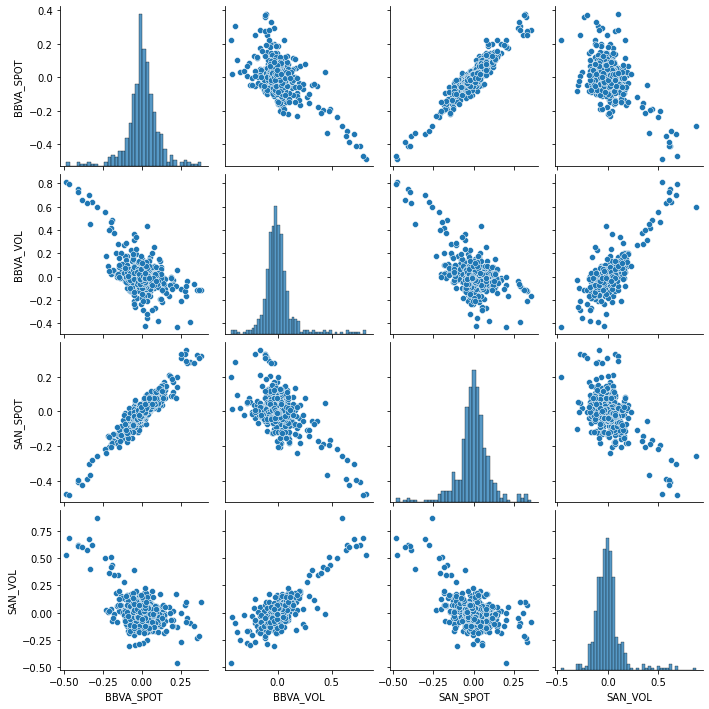
\includegraphics[width=0.7\textwidth]{Figures/MarketRisk/histdata.png}
\caption{Example of a parametric plot ($\sin (x), \cos(x), x$)}
\end{figure}


\subsection{Hedged Portfolio Problem}
\subsection{Converged vs non Converged Y}
\subsection{Transfer Learning}





